%! Author = niko
%! Date = 23/10/2023

% Preamble
\documentclass[../main]{subfiles}
\usepackage{glossaries}

% Document
\begin{document}

\chapter{The \tested{} educational test framework}\label{ch:tested-deel-1-tijdelijke-titel}

This chapter describes the internal mechanisms and workings of TESTed.
We begin by giving a brief introduction and consider some related work.
Then, we look at the architectural design of the TESTed framework.
We then consider the three parts of evaluating a submission:
the test suite, the evaluation process itself, and the generated feedback.
For the test suite, we look at the test suites as used internally by TESTed.
A more user-friendly format for test suites in TESTed-DSL, discussed in \cref{ch:tested-dsl}.
Then, we give a detailed overview of the evaluation process.
This is the process through which TESTed executes the test suite and determines the feedback that will be given on the submission.
Lastly, we briefly look at the feedback format.
Next, we describe how support for multiple programming languages is achieved.
We look at the internal API to give a good idea of what is required to support new programming languages.
Finally, we evaluate TESTed in educational practice.

This chapter is an expanded version of a previously published article:
\marginnote{This thesis doesn't have a word limit, so we can elaborate as much as we want.}
\par
\fullcite{strijbol_testededucational_2023}

\section{Introduction and background}\label{sec:introduction-and-background}

Formative feedback on solutions for programming exercises is a crucial part of learning to code~\autocite{shute_focus_2008,orrell_feedback_2006,luxton-reilly_introductory_2018}.
Feedback is most valuable and called formative if learners receive rich and qualitative feedback throughout the learning process.
Providing such feedback by hand is a challenge for educators since it is a time-consuming activity~\autocite{campos_multinational_2012, cheang_automated_2003, keuning_systematic_2018, hao_towards_2021, zavala_use_2018, staubitz_towards_2017, pirttinen_crowdsourcing_2018, gulwani_feedback_2014, tang_data-driven_2016, edwards_using_2004}.
The challenge is further exacerbated by a large number of students who work on multiple exercises~\autocite{camp_generation_2017, sax_examining_2017}.
Any laborious and time-consuming activity is a prime target for automation, and providing feedback is no different.
The computer science education field therefore has a long history of applying software test frameworks or general-purpose software tools (linters, formatters, etc.) on source code to automatically generate feedback~\autocite{hao_towards_2021, edwards_using_2004, paiva_automated_2022, keuning_systematic_2018}.

Off-the-shelf tools such as linters are low effort for educators, whereas software testing frameworks require an accompanying test suite for each individual programming exercise.
A test suite typically contains a set of tests that verify if the submission satisfies the requirements in the problem statement of the exercise.
This is similar to the practice of unit tests or integration tests in the software engineering field.
Beside general testing frameworks, computer science education also uses judge systems~\autocite{paiva_automated_2022, wasik_survey_2018}: specialized learning environments that provide rich feedback.
Defining an adequate test suite for an exercise is part of the reason why creating programming exercises is so time-consuming~\autocite{zavala_use_2018, staubitz_towards_2017, queiros_pexil_2011, pirttinen_crowdsourcing_2018, gulwani_feedback_2014, tang_data-driven_2016}.

An apparent solution to reduce the amount of time needed to create programming exercises is to create fewer exercises.
To achieve this without reducing the number of exercises available to students, maximal reuse of existing exercises is necessary.
Existing solutions to facilitate reusing exercises include standard formats in which exercises are written~\autocite{paiva_yet_2020, verhoeff_programming_2008}, open repositories with exercises~\autocite{staubitz_towards_2017}, or tools to convert between existing exercise formats~\autocite{queiros_babeloextensible_2013}.
However, reusing exercises remains difficult, particularly when attempting to reuse exercises across programming languages.
In existing judge systems, exercises are tightly coupled to the programming language in which the test suite is written.
Alternatively, test suites without such a tight coupling impose stringent restrictions on exercise specifications, e.g.\ only reading from stdin and writing to stdout.
Because of these restrictions, they often generate feedback of a lower quality than programming-language specific test suites.

To reuse programming exercises written for another programming language, exercise designers first have to learn a new test framework for that programming language.
Then, they have to write a new test suite for the exercise according to the specifications of the new test framework.
Alternatively, due to the vast number of programming languages~\autocite{bissyande_popularity_2013}, it might be necessary to implement a new test framework to support educational software testing, which is no small undertaking.

We focus on facilitating easy reuse of programming exercises across programming languages.
Our contributions include defining requirements for a test framework to support multiple programming languages, without imposing strict restrictions on programming exercises.
We also introduce TESTed, a proof-of-concept of a system that satisfies these requirements.
TESTed directly supports multiple programming languages for the same exercise, meaning the conversion of exercises to multiple test frameworks is no longer needed.
Exercise designers working on exercises for a single programming language can also benefit from TESTed, as it no longer forces them to learn new test frameworks for each new target language.
Finally, implementing support for new programming languages in TESTed is less work than implementing a complete test framework for each individual language, reducing the software development and maintenance cost dramatically.

\subsection{Related work}\label{subsec:related-work}

Since the terminology related to automated feedback on programming exercises is not used consistently within the field,
we begin by defining the terms used in this manuscript.
A programming exercise is the combination of a \textbf{problem statement} and a \textbf{test suite}.
When students attempt to solve the exercise using the instructions from the problem statement, they create a \textbf{submission} for the exercise.
The test suite is used by a judge system to \textbf{evaluate} the submission.
This results in \textbf{feedback} that is shown to the student.

We consider it useful to split a judge system into a \textbf{judge platform} and a \textbf{test framework}.
A judge platform is the graphical user interface that allows students and educators to upload and store submissions, display feedback, organize exercises into courses, and so on.
A test framework is responsible for generating feedback, by executing and evaluating submissions based on an exercise-specific test suite.
In existing literature, the distinction between these two is not always made, nor is it always relevant.
For example, some review manuscripts~\autocite{keuning_systematic_2018, wasik_survey_2018} or individual tools~\autocite{bez_uri_2014, petit_jutgeorg_2018} consider the entire system as a whole.
Other manuscripts focus specifically on judge platforms~\autocite{gusukuma_pedal_2020, striewe_architecture_2016}.
However, we believe this distinction is relevant for this manuscript, as evaluating submissions (the test framework) has a separate set of challenges compared to judge platforms (e.g.\ displaying feedback in a constructive way).
This manuscript focuses on test frameworks.

In educational contexts, software testing frameworks typically use either \textbf{output comparison} or \textbf{unit testing}~\autocite{paiva_automated_2022} to evaluate submissions.
Programming language support of test frameworks generally depends on the approach they adopt.
With unit testing, the test suite is often written in the same programming language as the submission, e.g.\ with tools based on xUnit~\autocite{meszaros_xunit_2007}.
Since the test suite is often written in the same programming language as the submission, it has full access to the submission.
The test suite can use function calls, data structures (e.g.\ lists, maps), primitive data types (e.g.\ integers, strings), examine return values, exceptions, runtime inspections (e.g.\ reflection), etc.
As a result, the test suite is tightly coupled to a specific programming language.
Evaluating a submission for the same exercise in another programming language would require a new test suite, often also involving another test framework.

With output comparison, the judge system imposes stringent restrictions on the programming exercise: only stdin, stdout, stderr and files can be used for input and output.
Prominent examples are the test frameworks used in ICPC-style (\emph{International Collegiate Programming Contest}, sometimes still referred to as ACM-ICPC)~\autocite{noauthor_icpc_2020} programming contests.
While this approach makes test suites independent of any programming language, the restrictions yield that testing is limited to data passed through stdin/stdout/stderr or via files.
All aspects of the submission that the test suite needs to check must be converted to a textual representation.
Files can contain binary data, but the same limitations apply.
Another disadvantage is the lack of granular testing: with these systems, tests are limited to the program as a whole.
It is, for example, not possible to add distinct tests for different functions inside the same program without obligating students to artificially split the program.

\section{Programming-language-agnostic test frameworks}\label{sec:programming-language-agnostic-test-frameworks}

Intuitively, an ideal test framework that supports multiple programming languages is a test framework with the testing capabilities of unit testing and the programming language support of output comparison.
First, we define the requirements a framework needs to satisfy to achieve this.
We also look at the consequences of those requirements on the framework.
We call a test framework that satisfies these requirements a \emph{programming-language-agnostic test framework}.

The \textbf{first framework requirement} is that test suites must be programming language independent.
A test suite must be usable to evaluate submissions in every programming language supported by the framework, without making changes to the test suite or adding languages-specific tests to it.
As a consequence of this requirement, adding support for new programming languages to the test framework must not demand changes to existing test suites.
All existing test suites must work with the new programming language without changes.

The \textbf{second framework requirement} is similar testing capabilities as unit testing.
Some concrete examples of what should be possile are:

\begin{itemize}[noitemsep]
    \item Provide textual input to stdin and reading output from stdout.
    \item Call functions implemented in submissions, and pass arguments to those functions.
    \item Evaluate values returned from function calls (with data type support).
    \item Create objects (constructors) and manipulate them (methods).
    \item Capture and evaluate other side effects such as exceptions, exit codes or files (or other persistent storage such as databases).
    \item Support exercises with deterministic/non-deterministic (e.g.\ random) behavior.
\end{itemize}

Support for these two requirements should not have disproportionately large drawbacks.
Therefore, we also consider the following soft requirements for a programming-language-agnostic test framework:

\begin{itemize}
    \item Configuring or creating exercises using the framework should not be significantly more difficult than configuring exercises using a language-specific test framework.
    \item Runtime and memory overhead should be minimal: the framework cannot be unacceptably slow or have a large memory footprint compared to a language-specific test framework. Providing feedback to students in a timely manner is important.
    \item Submissions should follow their language-specific conventions as closely as possible. For example, we want to support asynchronous and synchronous functions in JavaScript, or top-level functions should be implemented as a static function in Java, but not in Python or Kotlin that have proper support for top-level functions.
    \item Adding support for new programming languages to the framework should ideally be faster than implementing language-specific test frameworks for those languages, due to the ability to reuse shared parts of the implementation.
\end{itemize}


\section{Architectural design of the framework}\label{sec:conceptual design}

\begin{figure}[t]
    \centering
    \includestandalone{concept}
    \caption{
        Architectural design of TESTed, with colors indicating different programming languages.
        The framework consists of a set of Python packages and modules.
        These can be categorized as the core package and a set of programming-language-specific modules.
        The input for TESTed consists of a test suite, together with a submitted solution in one of the supported languages
        The output is the generated feedback.
    }
    \label{fig:conceptual-design}
\end{figure}

Our implementation of a programming-language-agnostic test framework is TESTed.
It implements these requirements using code generation.
This means that TESTed converts the test suite on the fly suite into the programming language of the submission.
It also takes care of the various aspects of the evaluation process: compiling the submitted code, executing the submission together with the test code, interpreting the results, and generating feedback.

While some parts of the evaluation process are programming-language-specific by necessity, such as generating the test code, a lot of parts are not.
For example, creating an execution plan or interpreting the test results and generating the feedback are not specific to any one programming language.
Therefore, the language-specific aspects are isolated in language modules, as illustrated in~\cref{fig:conceptual-design}.

\leavevmode\marginnote{
    A Python module is a \texttt{.py} file, while a Python package is a folder containing modules.
}%
TESTed is written in Python and organized into a set of Python modules and packages.
An import package is the \emph{core} package, which contains modules that are responsible for all language-independent tasks, such as scheduling tests.
This is discussed in \cref{subsec:execution-planning}.
In most cases, the core is also responsible for checking the collected test results and generating the feedback.
This is discussed in \cref{subsec:checking-results}.

All aspects that are specific to one programming language are bundled in one package.
These language-specific modules take care of all language-specific tasks, such as compiling submissions, executing submissions, and handling language-specific data types, expressions, and statements.
Since the language-specific code is limited to these modules, this offers benefits for adding support for new programming languages to TESTed, see \cref{sec:programming-language-support}.

TESTed requires a test suite for a programming exercise and a possible solution that needs to be evaluated as input.
The structure of the test suite is discussed in-depth in \cref{sec:test-suites}.
As a result of its evaluation, TESTed outputs a feedback report as has been illustrated with some examples
TODO.

\section{Test suites}\label{sec:test-suites}

As mentioned previously, TESTed-DSL (\cref{ch:tested-dsl}) is the intended way for exercise authors to create exercises for TESTed.
However, it is also possible to write JSON test suites.
These test suites are a direct JSON representation of the internal structure of a test suite as used by TESTed.
While JSON test suites have some advantages, such as being more flexible in some ways, they are also much more verbose and not guaranteed to stay stable.

In general, as the JSON test suite is a reflection of the internal structure, it is used as-is.
This means no processing is done: the test suite must be fully ``rolled out''.
For example, only the lowest levels of the test suite (the tests) can have options in the JSON suite.

A snippet of a test suite in JSON that is given in \cref{lst:expanded-json-test-suite}.
Note that the structure elements (tabs and contexts) are omitted in this example.

\begin{listing}
    \begin{minted}{json}
{
 "variable": "a_list",
 "type": "sequence",
 "expression": {
  "type": "sequence",
  "data": [
   {"data": 1, "type": "integer"},
   {"data": 2, "type": "integer"},
   {"data": 3, "type": "integer"},
   {"data": 2, "type": "integer"}
  ]
 }
}, {
 "input": {
  "type": "function",
  "name": "remove_all_occurences",
  "arguments": [
   "a_list",
   {"data": 2, "type": "integer"}
  ]
 },
 "output": {
  "result": {
   "value": {
    "type": "sequence",
    "data": [
     {"data": 1, "type": "integer"},
     {"data": 3, "type": "integer"}
    ]
}}}}
    \end{minted}
    \caption[]{
        A snippet of a JSON test suite for TESTed with two statements:
        \begin{enumerate*}[label=\emph{\roman*})]
            \item declaration of a variable (\texttt{aList}) that is assigned a sequence containing four integers 1, 2, 3, and 2 and
            \item call of the function \texttt{remove\_all\_occurrences} with two arguments: \texttt{aList} and the integer 2.
        \end{enumerate*}
        The expected return value is a list containing the integers 1 and 3.
    }
    \label{lst:expanded-json-test-suite}
\end{listing}

\subsection{Structure of a test suite}\label{subsec:structure-of-a-test-suite}

A test suite for TESTed is a hierarchical structure with three levels:

\marginnote{
    In this thesis, we use the Dodona naming scheme of the levels.
    However, TESTed supports an alternative, which is more in line with the naming schemes used in the literature: tabs, contexts, testcases, and tests are called \textbf{units}, \textbf{testcases}, \textbf{tests}, and \textbf{scripts} respectively.
    The overlap in terminology is unfortunate.
}

\begin{enumerate}
    \item \textbf{Tabs} are the top-level grouping mechanism.
    It allows grouping of logically related testcases together.
    \item \textbf{Contexts} are the basic building blocks of a test suite.
    A context is a set of dependent testcases.
    Contexts are independent of each other.
    \item \textbf{Testcases} are the lowest level.
    A testcase consists of some input and a series of checks about different side effects or results (i.e.\ return values, standard out, standard error, exit codes or exceptions).
    Each output check is also called a \textbf{test}.
\end{enumerate}

This structure mirrors the output generated by TESTed (see \cref{sec:tested-and-dodona}).
For example, the executed input for each test is also included in the output.
A possible visualization of these levels is given in~\cref{fig:dodona}, which shows the output rendered in Dodona~\autocite{van_petegem_dodona_2022}.

\begin{figure}
    \centering
    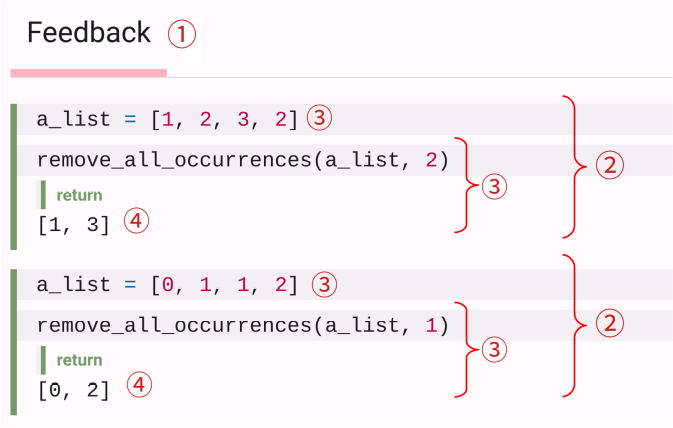
\includegraphics[scale=0.4]{dodona-rendering}
    \caption{A way to visually render the feedback (as done in Dodona) resulting from evaluating a submission (in Python) with the test suite from \cref{lst:expanded-json-test-suite}. There are four levels: \CircledText{1} tabs, \CircledText{2} contexts, \CircledText{3} units, and \CircledText{4} the tests. Here, each context consists of two testcases, the first of which has no tests, while the second has one test (the expected return value).}
    \label{fig:dodona}
\end{figure}

\subsection{Data serialization}\label{subsec:data-serialization}

TESTed uses data serialization to convert between the language-independent format of the test suite, and the generated test code.
Additionally, the same data serialization is used to convert return values from the submission into the language-independent format for checking (as described in \cref{subsec:checking-results}).

\begin{table}
    \caption{
        Overview of the basic types of TESTed and their implementation in the programming languages supported by TESTed.
        Sometimes, another type is used instead, based on the value. For example, an integer that is too large for \texttt{int} in Java will become a \texttt{long}.
        A dash (-) is used to indicate that the programming language does not support this type.
    }
    \label{tab:tested-basic-types}
    \begin{wide}
        \small\setlength{\tabcolsep}{0.25\tabcolsep}%
        \begin{tabular}{|l|l|l|l|l|l|l|l|l|}
            \hline
            \tested{} & Python         & JavaScript       & Java             & Kotlin           & Haskell          & C               & Bash          & C\#                 \\
            \hline
            integer   & \texttt{int}   & \texttt{number}  & \texttt{int}     & \texttt{Int}     & \texttt{Int}     & \texttt{int}    & -             & \texttt{Int32}      \\
            real      & \texttt{float} & \texttt{number}  & \texttt{double}  & \texttt{Double}  & \texttt{Double}  & \texttt{double} & -             & \texttt{Double}     \\
            boolean   & \texttt{bool}  & \texttt{boolean} & \texttt{boolean} & \texttt{Boolean} & \texttt{Bool}    & \texttt{bool}   & -             & \texttt{Boolean}    \\
            text      & \texttt{str}   & \texttt{String}  & \texttt{String}  & \texttt{String}  & \texttt{String}  & \texttt{char*}  & \texttt{text} & \texttt{string}     \\
            sequence  & \texttt{list}  & \texttt{array}   & \texttt{List}    & \texttt{List}    & \texttt{{[}{]}}  & -               & -             & \texttt{List}       \\
            set       & \texttt{set}   & \texttt{Set}     & \texttt{Set}     & \texttt{Set}     & -                & -               & -             & \texttt{Set}        \\
            map       & \texttt{dict}  & \texttt{object}  & \texttt{Map}     & \texttt{Map}     & -                & -               & -             & \texttt{Dictionary} \\
            nothing   & \texttt{None}  & \texttt{null}    & \texttt{null}    & \texttt{null}    & \texttt{Nothing} & \texttt{void}   & -             & \texttt{void}       \\
            \hline
        \end{tabular}
    \end{wide}
\end{table}

Each literal value is described by an object with two attributes: a value (e.g.\ the number \texttt{5.3}) and a data type (e.g.\ \texttt{real}).
These attributes are combined into a JSON object with two fields.
The value is encoded using the closest representation available in JSON\@.
For example, a number is represented by a JSON number, and a string is represented by a JSON string.
The data type of a literal value is more complex, since TESTed targets multiple programming languages that each support their own collection of data types.
TESTed therefore defines a set of rules to denote data types and their support in programming languages.
This allows TESTed to convert types between programming languages.

TESTed uses two categories of data types.
The first category is a limited set of \textbf{basic types} that are abstract and map to concepts.
Currently, the following basic types are supported:

\begin{description}[noitemsep]
    \item[\texttt{integer}] An integer.
    \item[\texttt{real}] A real number.
    \item[\texttt{boolean}] A Boolean value.
    \item[\texttt{text}] Textual data (e.g.\ strings).
          The intention is important here: for example, an \textsc{ASCII} character can be represented as both an integer or as text.
    \item[\texttt{sequence}] An ordered sequence of values.
    \item[\texttt{set}] An unordered collection of unique values.
    \item[\texttt{map}] A collection of key-value pairs, where the keys are unique.
    \item[\texttt{nothing}] A representation of ``nothing'', meaning no value.
    \item[\texttt{any}] \marginnote{The \texttt{any} type acts roughly as the \emph{top type}, except that we do not have a formal type system, nor do we have subtypes.} Any or unknown data type. This type is not usable in test suites, but is used to indicated return values of an unknown type.
\end{description}

When a test suite contains a literal value of a basic type, it will be serialized as an object of an actual data type in the target programming language.
An overview of all basic types and their implementation is given in \cref{tab:tested-basic-types}.
For example, a literal value with data type \texttt{map} will become a \texttt{Map} in Java or a \texttt{dict} in Python.

The second category consists of \textbf{advanced types}, which are more detailed or programming language specific.
Each advanced type is associated with a basic type, acting as a fallback.
For example, \texttt{int64} is an advanced type with the basic type \texttt{integer} as a fallback.

If a programming language does not support a particular advanced type, the corresponding basic type will be used.
For example, consider tuples.
Many programming languages do not have direct support for tuples, but exercises using tuples can still be solved by using the corresponding basic type (sequence).
For a concrete example, an exercise using a \texttt{tuple} can be solved in Java by using a \texttt{List}.

When adding a programming language, it is possible to disable this fallback for certain types.
For example, JavaScript has no support for fixed precision numbers.
This prevents TESTed from evaluating submissions in JavaScript if fixed precision numbers are used in the test suite.
TESTed will generate an appropriate error in this case.

Currently supported advanced types are:

\begin{description}[noitemsep]
    \item[\texttt{int8}] 8-bit integers (signed)
    \item[\texttt{uint8}] 8-bit natural numbers (unsigned)
    \item[\texttt{int16}] 16-bit integers (signed)
    \item[\texttt{uint16}] 16-bit natural numbers (unsigned)
    \item[\texttt{int32}] 32-bit integers (signed)
    \item[\texttt{uint32}] 32-bit natural numbers (unsigned)
    \item[\texttt{int64}] 64-bit integers (signed)
    \item[\texttt{uint64}] 64-bit natural numbers (unsigned)
    \item[\texttt{bigint}] integers without upper and lower limit (signed)
    \item[\texttt{single\_precision}] single precision real number
    \marginnote{The names for real numbers are borrowed from IEEE 754.}
    \item[\texttt{double\_precision}] double precision real number
    \item[\texttt{double\_extended}] double extended precision real number
    \item[\texttt{fixed\_precision}] fixed precision real number
    \item[\texttt{array}] a mutable fixed-size sequence
    \item[\texttt{list}] a mutable variable-size sequence
    \item[\texttt{tuple}] an immutable sequence
    \item[\texttt{char}] a single character
    \item[\texttt{undefined}] \texttt{undefined} in JavaScript
    \item[\texttt{null}] \texttt{null} in JavaScript
\end{description}

The advanced data types are also where the language-specific aspects can come into play.
For example, in addition to the basic type \texttt{nothing}, we have both \texttt{undefined} and \texttt{null}.
In most languages, there is no difference between those, but for example, in JavaScript there is.
Having both available as an advanced type allows exercises to use either in JavaScript exercises, while still being language-agnostic.

An overview of the supported advanced types for each programming language is given in \cref{tab:tested-advanced-types}.
A plus sign (+) in a column indicates that the programming language has limited support for the data type.
This means that the programming language will fall back to the basic type (as discussed previously).
A dash means there is no support in the programming language: exercises using this data type will not be solvable in that programming language.

\begin{table}
    \caption{
        An overview of advanced types supported by TESTed.
        The first column contains all advanced types, and the second column contains their corresponding basic type.
        The other columns contain the mapping to the data types of the programming languages currently supported.
        Note that the table is split into two.
    }
    \begin{wide}
        \small\setlength{\tabcolsep}{0.5\tabcolsep}%
        \begin{tabular}{|l|l|l|l|l|l|l|l|l|}
            \hline
            \tested{}         & Basic & Python         & JavaScript       & Java             & Kotlin   \\
            \hline
            int8              & integer & + & + & \texttt{byte} & \texttt{Byte} \\
            uint8             & integer & + & + & + & \texttt{UByte} \\
            int16             & integer & + & + & \texttt{short} & \texttt{Short} \\
            uint16 & integer & + & + & + & \texttt{UShort} \\
            int32 & integer & + & + & \texttt{int} & \texttt{Int} \\
            uint32 & integer & + & + & + & \texttt{UInt} \\
            int64 & integer & + & + & \texttt{long} & \texttt{Long} \\
            uint64 & integer  & + & + & + & \texttt{ULong} \\
            bigint & integer  & \texttt{int} & \texttt{BigInt} & \texttt{BigInteger}
            & \texttt{BigInteger} \\
            single\_precision & real & + & + & \texttt{float} & \texttt{Float} \\
            double\_precision & real & + & + & \texttt{double} & \texttt{Double} \\
            double\_extended & real & + & + & + & + \\
            fixed\_precision & rational & \texttt{Decimal} & - & \texttt{BigDecimal}
            & \texttt{BigDecimal} \\
            array & sequence & + & + & \texttt{array} & \texttt{Array} \\
            list & sequence & \texttt{List} & + & \texttt{List} & \texttt{List} \\
            tuple & sequence & \texttt{Tuple} & + & + & + \\
            char & text & + & + & \texttt{char} & \texttt{Char} \\
            undefined & nothing & + & \texttt{undefined} & + & + \\
            \hline
        \end{tabular}
        \begin{tabular}{|l|l|l|l|l|l|l|l|l|}
            \hline
            \tested{}         & Haskell                   & C                        & Bash & C\# \\
            \hline
            int8              & \texttt{Data.Int.Int8}    & +                        & -    & \\
            uint8             & \texttt{Data.Word.Word8}  & +                        & -    & \\
            int16             & \texttt{Data.Int.Int16}   & \texttt{short}           & -    & \\
            uint16            & \texttt{Data.Word.Word16} & \texttt{unsigned\ short} & -    & \\
            int32             & \texttt{Data.Int.Int32}   & \texttt{int}             & -    & \\
            uint32            & \texttt{Data.Word.Word32} & \texttt{unsigned\ int}   & -    & \\
            int64             & \texttt{Data.Int.Int64}   & \texttt{long}            & -    & \\
            uint64            & \texttt{Data.Word.Word64} & \texttt{unsigned\ long}  & -    & \\
            bigint            & \texttt{Integer}          & -                        & -    & \\
            single\_precision & \texttt{Float}            & \texttt{float}           & -    & \\
            double\_precision & \texttt{Double}           & \texttt{double}          & -    & \\
            double\_extended  & -                         & \texttt{double\ double}  & -    & \\
            fixed\_precision  & -                         & -                        & -    & \\
            array             & -                         & -                        & -    & \\
            list              & \texttt{{[}{]}}           & -                        & -    & \\
            tuple             & \texttt{()}               & -                        & -    & \\
            char              & \texttt{Char}             & \texttt{char}            & +    & \\
            undefined         & +                         & +                        & -    & \\
            \hline
        \end{tabular}
    \end{wide}
    \label{tab:tested-advanced-types}
\end{table}

\section{Evaluating submissions}\label{sec:evaluating-submissions}

The input for the evaluation process is a test suite and a submission, which is typically provided by the judge platform in which TESTed runs (or can be provided manually if TESTed is run on the command line).
A general overview is given in~\cref{subsec:evaluation-process}.
Other subsections dive into more detail of individual parts of the process.

\subsection{The complete evaluation process}\label{subsec:evaluation-process}

A schematic overview of the complete evaluation process used by TESTed when evaluating a submission is \cref{fig:flow}.
The very first step in the evaluation process is checking if the exercise is solvable in the programming language of the submission (see~\cref{subsec:solvability-and-correctness-checks}).
Next, in the first step of the actual evaluation, the test suite is partitioned into compilation and execution units, as described in~\cref{subsec:execution-planning}.
For each of these units, the relevant code is generated and the resulting test code is compiled, as explained in~\cref{subsec:code-generation}.
The code is generated in the programming language of the submission.
This code generation is the bulk of language-specific code in TESTed, whose design and implementation are discussed in \cref{sec:programming-language-support}.

After compilation, each resulting executable contains one or more execution units.
These are then all executed, and the side effects (such as exceptions, stdout, stderr, etc.) and results (i.e.\ return values) are recorded.
These results are then checked for correctness against the test suite (\cref{subsec:checking-results}).
This results in the feedback, which is returned by TESTed.

TESTed also has a step where static analysis is possible on the submission.
\marginnote{Examples include \texttt{ESLint}, \texttt{pylint} or \texttt{hlint}.}
Currently, all supported programming languages use this step to run a linter on the submission, the results of which are also included in the feedback as code annotations (\cref{subsec:static-analysis-of-the-submission}).

\begin{figure}
    \centering
    \includestandalone{flow}
    \caption{
        The evaluation process of TESTed.
        The input consists of a submission and a test suite.
        After the planning phase, test code is generated, compiled, and executed.
        These results are then checked, which produces the final feedback.
        Separately, a linter runs on the submission, and its results are also included in the feedback.
    }
    \label{fig:flow}
\end{figure}

\subsection{Solvability and correctness checks}\label{subsec:solvability-and-correctness-checks}

The first step in the evaluation process is checking if the test suite is usable for the programming language of the submission.
This might not be the case for a number of reasons, the three main ones being:

\begin{itemize}
    \item The exercise designer has limited in which programming languages the exercise may be solved.
    \item The test suite uses constructs that are not supported by the programming language of the solution.
          For example, if the test suite uses object-oriented programming, the exercise will not be solvable in C or Haskell.
    \item The test suite contains programming-language-specific code but does not provide code for the programming language of the submission.
          For example, it is possible to manually provide the test code.
\end{itemize}

Additionally, there are some correctness checks, for example, on the syntax of the test suite.

\subsection{Execution planning}\label{subsec:execution-planning}

The next step is planning the execution of the evaluation.
As discussed before, a test suite contains a number of testcases, which must be independent of each other.
This allows TESTed to implement optimisations to improve performance.

TESTed partitions the test suite into compilation units (a set of testcases that are compiled together), which are in turn partitioned into execution units (a set of testcases that are executed together).
While different compilation units cannot be executed as one execution unit, it is possible that one compilation unit represents multiple execution units.

\begin{figure}
    \begin{subfigure}{\textwidth}
        \centering
        \includestandalone{planning-1}
        \caption{
            A schematic representation of the test suite.
            The test units are represented with green boxes, while the testcases (denoted as C\textsubscript{$n$}) are black boxes.
            In the subsequent figures, we leave the test suite box out to simplify the image.
        }
        \label{fig:planning-suite}
    \end{subfigure}
    \par\bigskip
    \begin{subfigure}{\textwidth}
        \centering
        \includestandalone{planning-2}
        \caption{
            The two possibilities for compilation units (denoted by red boxes).
            The upper scheme (with one compilation for the whole test suite) is always tried first.
            If this fails, each test unit becomes a compilation unit (the red boxes thus overlap with the green ones in the figure).
        }
        \label{fig:planning-compilation}
    \end{subfigure}
    \par\bigskip
    \begin{subfigure}{\textwidth}
        \centering
        \includestandalone{planning-3}
        \caption{
            Two possibilites execution unit partitionings (denoted by blue boxes), depending on the compilation units.
            In the first paritioning, there is a single compilation unit that is split into three execution units.
            The second partitioning cannot use the same execution units, as an execution unit cannot comprise multiple compilation units.
        }
        \label{fig:planning-execution}
    \end{subfigure}
    \caption{Schematic representation of the planning steps.}
\end{figure}

\subsubsection{Performance impact of the planning}

If performance was not relevant, the easiest execution plan would be to compile and execute each testcase individually.
After all, they are independent of each other, and separate compilation and execution would ensure that independence.

However, this would be prohibitively slow: a test suite with fifty test cases would need fifty compilation steps and fifty execution steps.
Creating an execution plan is thus intended to improve performance, which is done in two ways:

\begin{enumerate}[noitemsep]
    \item Reducing the number of compilation units.
    \item Reducing the number of execution units.
\end{enumerate}

\subsubsection{Compilation units}
\label{subsubsec:compilation-units}

First, TESTed tries to use a single compilation unit for the whole test suite.
This is achieved by creating a program that accepts an argument to indicate the execution that should be run.

In programming languages without an explicit compilation step, the compilation is no more than a syntax check.
\marginnote{
    For example, our JavaScript implementation uses \texttt{node -c}.
}
In compiled languages, the compilation is often much stricter, for example, failing if a non-existing function is used.

Techniques used to improve performance must be weighed against the usability.
For example, consider an exercise where students must implement two or three functions.
Students might implement the first function and submit their solution.
With a single compilation unit, a compilation would occur, since our test code calls functions that do not exit.
This will prevent the first function from being evaluated, even if it was correct.

To prevent this, if the compilation of the whole test suite fails, TESTed falls back to using one compilation unit per unit in the test suite.
These two approaches are illustrated in~\cref{fig:planning-compilation}.

This is why a unit is intended to be a set of logically related testcases.
Continuing with the example from before, there might be a separate unit for each function the exercise requires.
Going more fine-grained, that is compiling each testcase individually, does not seem useful.
While potentially providing faster feedback, the performance impact is not worth it.

Compiling at the unit level is a good compromise between fain-grained compilation (thus allowing more of the submission to be evaluated) and performance (the more compilation units, the slower the evaluation will be).

\subsubsection{Execution units}

Next, the compilation units from the previous steps are partitioned into execution units.
\marginnote{
All programming languages, including the non-compiled ones, are handled the same way.
This allows the most consistency between programming languages.
}
Each execution unit can be at most one compilation unit: we cannot execute multiple compilation units together,
as each compilation unit results in a separate executable.
However, depending on the testcases inside a compilation unit, we can (and do) execute a compilation unit multiple times.

For performance reasons, the ideal partitioning would be a single execution unit for the whole test suite.
However, this prevents certain types of exercises from being evaluated correctly.
Therefore, a new execution unit is started based on the type of testcase: if a testcase has stdin, command line arguments, or an explicit check for the exit code, a new execution unit is started.

\subsection{Generating test code}\label{subsec:code-generation}

Depending on the execution plan, the appropriate code is generated for the test suite.
In concept, this step converts the programming-language-independent test suite into actual source code, in the programming language of the test suite.
For example, for a submission in JavaScript, the generated code will also be in JavaScript.

As shown in~\cref{fig:flow}, code is generated for each compilation unit.
The main purpose of the generated code is to execute the tests specified in the test suite.
For this reason, we also call the generated code the \emph{test code}.

Besides executing the tests from the test suite, the generated code also contains some \emph{ceremonial} code required by TESTed.
Some examples of this code are:

\begin{itemize}
    \item As mentioned in~\cref{subsec:execution-planning}, in the ideal case, we only have one compilation unit and thus one executable for the whole test suite.
     We thus generate a wrapper that executes the correct execution unit based on some parameter (e.g.\ \texttt{./testcode "unit1"}).
    \item The generated code includes serialization capabilities (\cref{subsec:data-serialization}), to convert captured values into the internal data format used by TESTed.
    \item The tests are wrapped in code that captures side effects and values, such as exceptions, return values, etc.
\end{itemize}

This code generation is the main task of the programming-language-specific modules, discussed in \cref{sec:programming-language-support}.

\subsection{Executing test code}\label{subsec:executing-test-code}

After the test code has been generated and compiled into executables, these executables are then (as one would expect) executed.

During this execution, special care is taken to ensure that the executions are independent of each other.
As discussed in \cref{sec:tested-and-dodona}, execution happens in a special directory called the \emph{workdir} (from working directory).
For each execution, TESTed creates a new subdirectory and copies the relevant files into that subdirectory.
The execution then happens in the subdirectory.

The independence of execution is useful to prevent other executions from interfering.
For example, consider an erroneous submission for an exercise where data is provided in a file.
If the submission overwrites or changes the file by accident, subsequent executions would use the modified file.
However, since the file is copied into each subdirectory, this scenario is prevented.

A second benefit of the independent executions is the ability to execute in parallel.
However, even in that scenario, this improves the performance of certain exercises, for example those exercises that use scripts, command lines, or main functions.

The astute reader might wonder how this is implemented, since TESTed is written in Python, a language whose default implementation (CPython) has an infamous global interpreter lock (or GIL).
This means that at any one time, only one thread can execute Python code.
\marginnote{
Work is ongoing to improve the situation, or even remove the GIL, as PEP 703: \url{https://peps.python.org/pep-0703/}
}
One workaround is to use multiple processes: this sidesteps the issue entirely, but using multiple processes is fairly heavy in general.
This is even truer in TESTed, as executing the test code already happens in a separate process.

This leads directly to the solution in TESTed: since the test code is executed in a separate process, the GIL does not apply.
Most of the time is spent waiting on results from a subproces.

\subsection{Checking test results}\label{subsec:checking-results}

The code responsible for checking wheter test results (return values, stdout, etc.) are correct is called an oracle. TODO referentie.
TESTed supports three types of oracles, which can be divided into two categories.
The first two oracle types are generic, meaning that they are programming language independent.
These are also explained in \cref{subsec:checking-results}, where the focus lies on using the oracles.
The third oracle type is a programming-language-dependent oracle.

The two generic oracles are the built-in oracles and the programmed oracles.
The first are oracles are, as the name implies, built into TESTed.
These are rather simple, but should suffice for most exercises.
Currently, the following oracles are included:

\begin{itemize}
    \item The text oracle.
          This oracle compares two strings and is used for stdout and stderr.
          The oracle has some options, for example, to ignore trailing whitespace, to attempt to parse the text as floating point numbers or case sensitivity.
          The expected value can be provided either as a string, or as a file, in which case the contents of said file are used as the string.
    \item The file oracle.
          This allows comparison between two files, either comparing the whole file, or comparing the file line-by-line.
          When comparing line-by-line, the text oracle is used, so the same options can be provided.
    \item The return value oracle.
          This oracle compares two values (see TODO for the test values).
          The oracle does more than just a value comparison: the types of the data are also compared, using the TESTed type system (see TODO for how this works).
    \item The exception oracle.
          This allows checking exceptions.
          By default, only the message of the exception is checked, as the type of an exception is programming language dependent.
          However, the oracle does have an option to provide the expected type for the different programming languages, in which case those will be checked as well.
          Do note that checking the type happens with a string-based check, meaning that if a student implements a custom exception with the same name, it will pass the check.
\end{itemize}

There are a number of scenarios where the built-in oracles are not enough to properly check an exercise.
One such example is an exercise where dynamic data is used, for example a return value that depends on the current date.
Another example is a random or otherwise nondeterministic return value, where the value must satisfy some conditions.
Finally, sometimes the exercise is static, but you want to provide some exercise-specific feedback.
For example, if the exercise is to generate an SVG, you might want to show that SVG to students.

For these scenarios, a programmed oracle can be used.
Such an oracle is, in essence, an extension of the built-in oracles: instead of using a built-in oracle, TESTed will call the exercise-provided oracle.
See TODO for how to use such an oracle.

We have not yet encountered an exercise not covered by the generic oracles; however, it is not hard to imagine exercises that cannot be checked using those.
As such, TESTed provides an escape hatch: a programming-language-specific oracle.
These oracles are run together with the generated test code and skip the serialization pipeline.
They are therefore not subject to the serialization limits of TESTed.
An example could be an exercise where a function returns an instance of a custom class.

The big downside to using these oracles is that they are programming-language-specific.
The oracle thus has to be implemented in each programming language the exercise supports.
These oracles are therefore only provided as an escape route for language-specific expressions, statements, and data types.

\subsection{Static analysis of the submission}\label{subsec:static-analysis-of-the-submission}

TESTed also provides a way to perform exercise-independent static analysis on the submission as part of the evaluation process.
TODO: references naar linters en dat ze goed werken.
Currently, all supported languages (except C\#, where the compiler acts a linter) use an external linter to generate additional feedback, see~\cref{tab:linters}.
While this feedback is generally not specific to an exercise, nor is its main goal to check the correctness of the submission, it does provide additional hints to students on how to improve their submission.

TODO: refereren waar mogelijk
\begin{table}[h]
    \centering
    \caption{Overview of the used linters in TESTed.}
    \label{tab:linters}
    \begin{tabular}{|l|l|}
        \hline
        Programming language & Linter \\
        \hline
        Bash & Shellcheck  \\
        C & Cppcheck \\
        Haskell & HLint \\
        Java & Checkstyle \\
        JavaScript & ESLint \\
        Kotlin & Ktlint \\
        Python & Pylint \\
        \hline
    \end{tabular}
\end{table}

\subsection{Feedback}\label{subsec:feedback}

The last step of the evaluation process is to return the generated feedback.
The feedback format used by TESTed is the Dodona feedback format, which we discuss in \cref{subsec:dodona-output}.

\section{Programming language support}\label{sec:programming-language-support}

The parts of the evaluation process that are programming-language-specific are implemented using a module system.
To make adding new programming languages easy, TESTed enforces a strict separation of concerns with regard to programming-language-specific tasks.
All programming-language-specific actions and tasks must go through a single well-defined interface.
This interface is implemented using Python's object-oriented capabilities by defining an abstract base class (ABC) called \mintinline{python}{Language}.

This \mintinline{python}{Language} class has a set of abstract methods, for which an implementation is thus necessary, and the remaining optional methods, which may be overridden but are not required.
This abstract class is the interface between the core modules of TESTed and the language-specific modules.
No other modules have language-specific code.

The main task when adding support for a new programming language is to implement this abstract base class.
Some other smaller tasks are registering the language in TESTed and adding support in the test suite for this new programming language.

The remainder of this section describes the different methods that must or can be implemented.
We always begin by providing the signature, followed by a discussion of the method.
Most of this information is also available in the class itself as documentation in the code.

\subsection{Compilation}\label{subsec:impl-compilation}

\begin{minted}{python}
    def compilation(self, files: list[str]) -> CallbackResult:
\end{minted}

The compilation method must return the command that TESTed will use to compile the test code together with the submission.
The return type \mintinline{python}{CallbackResult} is an alias for \mintinline{python}{tuple[Command, list[str] | FileFilter]}.

The first value of the returned tuple is the compilation command.
This command is a list of strings, which will be executed with the Python \mintinline{python}{subprocess} package.
For generating this command, the \mintinline{python}{files} argument can be useful: it is a list of potential dependencies.
By convention, the last file in the list is the file containing the \emph{program entry point} (which is often a main function).

The second part of the return value must be a list of generated files, in which by convention the last file is the executable file.
All files in this list will be made available to the execution command in the next step of the evaluation process.
Alternatively, a file filter can be returned, which allows dynamic filtering of the resulting files after compilation.

As an example, consider the C language.
When compiling C, we are only interested in the resulting binary, which also has a predictable name.
The list of generated files can thus contain a single string: the name of the generated binary.

However, it is not always possile to predict the list of generated files, nor is it possible to predict their names.
For example, in Java, compiling a file will result in one or more class files, depending on the content of the Java file (a nested class will result in more class files).
In that case, the file filter can be used, which will be called for each file in the compilation directory after compilation has completed.

As a concrete example, this is how the method is called and what its return value is for C (on Windows):

\begin{minted}{pycon}
    >>> compilation(['submission.c', 'evaluation_result.c', 'context_0_0.c', 'selector.c'])
    (
        ['gcc', '-std=c11', '-Wall', 'evaluation_result.c', 'values.c', 'selector.c',
         '-o', 'selector.exe'], ['selector.exe']
    )
\end{minted}

The compilation method is optional: languages that do not require compilation can use the default implementation.
However, this step is ideal to at least perform a syntax check, and we recommend that all languages do this, if at all possible.
Even non-compiled languages often have a syntax checker that is faster than executing the program.
For example, both Python and JavaScript are not considered compiled languages, but both implement a syntax check in TESTed.

\subsection{Execution}\label{subsec:impl-execution}

One of the most important methods is the method responsible for creating the execution command.
This method is called after the compilation step, if that step was successful.

\begin{minted}{python}
    def execution(self, cwd: Path, file: str, arguments: list[str]) -> Command:
\end{minted}

This method must return one value: the command to execute.
As with the compilation method, the returned command will be executed by passing it to Python's \mintinline{python}{subprocess} package.

The returned command must execute the file from the \mintinline{python}{file} argument.
The argument \mintinline{python}{arguments} contains a list of command line arguments that must be passed to the program.
The \mintinline{python}{cwd} arguments is the directory in which the execution will take place.
This can be useful for languages that compile to a binary executable.
Since this executable is not on the path, it is safer to return an absolute path to it.

Continuing with the same example in C, a call to this method would look like this:

\begin{minted}{pycon}
    >>> execution('/test/path', 'executable.exe', ['arg1', 'arg2'])
    ['/test/path/executable.exe', 'arg1', 'arg2']
\end{minted}

All files that were included in the return value of the compilation method will also be available in the execution directory, in addition to other dependencies that we discuss next.

\subsection{Dependencies and other files}\label{subsec:dependencies-and-other-files}

In the commands from two previous sections, the methods receive a list of files that are potential dependencies for compilation or execution.
There are also some methods that optionally can influence which files are considered dependencies.

\begin{minted}{python}
    def initial_dependencies(self) -> list[str]:
\end{minted}

Returns a list of additional dependencies that will be included in the compilation and execution.
The returned strings are paths to files, relative to the implementation folder of the language module in TESTed.

For example, most languages include a separate file to deal with encoding return values into the TESTed data format.

\begin{minted}{python}
def filter_dependencies(self, files: list[Path], context_name: str) -> list[Path]:
\end{minted}

Used to filter the results of the compilation step to the files needed for one testcase.
In most cases, a single compilation step is used for all testcase.
However, not all languages need all resulting files for each execution.
By default, the name of the testcase is used to filter the files.

\begin{minted}{python}
def find_main_file(self, files: list[Path], name: str) -> tuple[Path | None, Status]
\end{minted}

This optional method finds the main file (i.e.\ the executable file or the file with the main method) in a list of dependencies.
The method should either return the path to that file with the status \texttt{CORRECT}, or return \mintinline{python}{None} with an error status if the file could not be found.
It can be useful if the normal convention of putting the main file last in a list of files is not enough.

\begin{minted}{python}
    def modify_solution(self, solution: Path):
\end{minted}

A callback that allows modifying the submission.
The submission should be modified in place.
The callback is called after linting, but before compilation or execution.

An example of this use case is JavaScript.
To support both CommonJS and ES6 modules, we analyze the code and add exports for all functions, variables, and classes in the submission.
Similarly, the main function in C programs is renamed to prevent conflicts with the main function in the generated TESTed code.

\subsection{Configuration and conventions}\label{subsec:configuration-and-conventions}

There are a number of simple methods that deal with the different conventions used by the programming language.

\begin{minted}{python}
    def get_string_quote(self):
\end{minted}

Returns the character used to quote strings.
By default, this is a double quotation mark (\texttt{"}).

\begin{minted}{python}
    def naming_conventions(self) -> dict[Conventionable, NamingConventions]:
\end{minted}

Returns the naming conventions used by the programming language.
It must return a dictionary, which maps different aspects to a naming convention.

The ``conventionable'' aspects are namespaces, function names, identifiers, properties, classes, and global identifiers.
Most are self-explanatory, except for namespace, whose meaning depends on the programming language.
In some languages this is used as the name for packages or modules, but in Bash, for example, it is used as the name of the script.
\Cref{tab:naming-conventions} contains an overview of the available naming conventions in TESTed.

\marginnote{
    In practice, most languages use camel case and snake case (and their uppercase variants).
}
\begin{table}[h]
    \centering
    \caption{Available naming conventions in TESTed.}
    \label{tab:naming-conventions}
    \begin{tabular}{|l|l|}
        \hline
        Naming convention & Example \\
        \hline
        Camel case & \texttt{thisIsAnExample}  \\
        Snake case & \texttt{this\_is\_an\_example} \\
        Camel snake case & \texttt{this\_Is\_An\_Example} \\
        Cobol case & \texttt{THIS-IS-AN-EXAMPLE} \\
        Dash case & \texttt{this-is-an-example} \\
        Donor case & \texttt{this|is|an|example} \\
        Flat case & \texttt{thisisanexample} \\
        Macro case & \texttt{THIS\_I\_AN\_EXAMPLE} \\
        Pascal case & \texttt{ThisIsAnExample} \\
        Pascal snake case & \texttt{This\_Is\_An\_Example} \\
        Train case & \texttt{This-Is-An-Example} \\
        Upper (flat) case & \texttt{THISISANEXAMPLE} \\
        \hline
    \end{tabular}
\end{table}

\begin{minted}{python}
    def file_extension(self) -> str:
\end{minted}

Return the main file extension for the programming language.
For language with multiple extensions, this should return the extension used for executable (main) files
For example, in C this returns \texttt{c} and not \texttt{h}.

\begin{minted}{python}
    def is_source_file(self, file: Path) -> bool:
\end{minted}

An optional method that determines if a file could be a source file for the programming language.
By default, this will check the extension of the file against the extension provided by the \mintinline{python}{file_extension} method.

\begin{minted}{python}
    def submission_file(self) -> str:
\end{minted}

Returns the name of the submission file.
By default, this calls the helper function \mintinline{python}{submission_name} and adds the file extension to it.

\subsection{Type support}\label{subsec:type-support}

The system for data types used by TESTed is explained in TODO.
The actual implementation of this system happens with the following methods.

\begin{minted}{python}
    def supported_constructs(self) -> set[Construct]:
\end{minted}

This method should return a set of the constructs that are supported by this language.
This is one of the mechanisms used in~\cref{subsec:solvability-and-correctness-checks} to check if a submissions in a certain programming language are possible for a given test suite.

The currently supported constructs are:

\begin{description}
    \item[Objects] Object-oriented constructs, such as classes.
    \item[Exceptions] Exception support.
    \item[Function calls] Function call support.
    \item[Assignments] The result of an expression can be assigned to a variable.
    \item[Heterogeneous collections] Data structures whose elements can be of different data types.
    \item[Default parameters] Parameters in a function with a default value.
    \item[Named arguments] Parameters in a function can be passed by name rather than (or in addition to) by position.
    \item[Global variables] Variables or constants defined at a top-level.
\end{description}

Note that the constructs can sometimes be interpreted in a loose sense.
For example, Haskell indicates that assignments are supported, even if this is not strictly true.
\mintinline{haskell}{x = 5 + 5} defines a new function \mintinline{haskell}{x} with the body \mintinline{haskell}{5 + 5}.
However, for practical purposes, this can fulfill the same role as an assignment in TESTed.

\begin{minted}{python}
    def map_type_restrictions(self) -> set[ExpressionTypes] | None:
    def set_type_restrictions(self) -> set[ExpressionTypes] | None:
\end{minted}

These two optional functions allow restricting which data types are allowed in map keys and sets respectively.
For example, in Python, a list is not hashable, meaning it cannot be used as the key in a dictionary, nor can it be an element of a set.

\begin{minted}{python}
    def datatype_support(self) -> dict[AllTypes, TypeSupport]:
\end{minted}

This function is used to indicate the data type support for the language, as described in X.
The return value is a mapping of the types to their support.
The default is unsupported: only supported types must be present.

For example, in Bash, the implementation of this function looks like:

\begin{minted}{python}
    def datatype_support(self) -> dict[AllTypes, TypeSupport]:
        return {
            AdvancedStringTypes.CHAR: TypeSupport.REDUCED,
            BasicStringTypes.TEXT: TypeSupport.SUPPORTED,
        }
\end{minted}

Strings are supported (and are the only type supported by TESTed).
Characters are supported, but in reduced form.
This means that strings will be used for characters.

\subsection{Stacktraces and compiler outputs}\label{subsec:error-messages-and-compiler-outputs}

In most cases, stacktraces from errors, compiler errors, or compiler warnings contain lines referring to the generated TESTed code.
However, these lines are not relevant nor useful to students.
Therefore, these methods provide a way to clean up stacktraces.

Another example of a use-case for these is adding links in the feedback to the relevant lines in the submission.
Dodona also supports this feature, so users there can click on a stacktrace and go to the relevant lines, like some IDEs.

\begin{minted}{python}
    def compiler_output(self, stdout: str, stderr: str) -> tuple[list[Message], list[AnnotateCode], str, str]
\end{minted}

Allows cleaning up the output from the compiler.
The returned tuple contains a list of messages, a list of code annotations, and the clean version of the compiler output.

\begin{minted}{python}
    def cleanup_stacktrace(self, stacktrace: str) -> str:
\end{minted}

Cleans up a stacktrace.

\subsection{Code generation}\label{subsec:code-generation2}

As mentioned in \cref{subsec:code-generation}, TESTed works by generating code.
The following methods are called on the language module to generate code for various language constructs.
In the implementation for most languages, the code generation is implemented in a separate module, and these methods just call that module.

\begin{minted}{python}
    def generate_statement(self, statement: Statement) -> str
\end{minted}

Generate code for a statement.

\begin{minted}{python}
    def generate_execution_unit(self, execution_unit: "PreparedExecutionUnit") -> str:
\end{minted}

Generate code for an execution unit.
Of course, it is expected that the implementation of this method uses the other methods for generating code.
For example, an execution unit probably needs to generate code for a statement somewhere, which would be done using \mintinline{python}{generate_statement}.

When generating the code for an execution unit, a few things must be taken into account (\cref{fig:generated-code}):

\begin{itemize}
    \item TESTed expects two secret sentinel values to be present in all outputs (stdout, stderr, return values, exceptions): \texttt{testcase\_separator\_secret} between the outputs for tests and \texttt{context\_separator\_secret} between the outputs for testcases.
    \item Return values and exceptions must be serialized in JSON, using the internal data form from TESTed.
    \item The generated code should be robust against unexpected output, including exceptions.
\end{itemize}

\begin{figure}
    \centering
    \includestandalone{code-generation}
    \caption{Overview of code generation in TESTed.
        In the optimal scenario, a single executable is generated and compiled for the whole test suite.
        Its main function has one job: selecting the correct function for the relevant execution unit.
        This is illustrated here with a \mintinline{java}{switch}.
        Each of these execution functions will write a separator to all outputs (return values, stdout, stderr, exceptions) and will then call the function for the contexts in that execution unit.
        This function for the context does something very similar: it writes the context separator to the outputs and execute the testcases.
        The final results for each output are a set of captured values separated by the context and testcase separators.
    }
    \label{fig:generated-code}
\end{figure}


\section{\tested{} and Dodona}\label{sec:tested-and-dodona}

Dodona (TODO: cite) is an online platform for solving and submitting programming exercises.
It is developed by Team Dodona (of which I am a part) at Ghent University, originally for use in our own courses.
However, the platform has enjoyed a wide adoption within Flanders, and is now used by over a thousand colleges, universities, and schools.
While TESTed is available as a standalone tool, it was primarily developed with Dodona in mind.
Therefore, some design decisions made by the Dodona platform still apply to TESTed as well.

In Section TODO, we have already made a distinction between a platform and the judge.
Some other platforms (and accompanying judges) are discussed in TODO.

In this section, we briefly discuss the relevant aspects of Dodona that have an impact on TESTed.
We also look at Dodona's feedback format, which is also used by TESTed.

\subsection{Architecture}

A relatively unique aspect of Dodona is the complete separation of the platform code and the judge code.
The platform code is the web application and responsible for almost everything, from classroom management, to rendering web pages with the user interface used by students and teachers.
The judge is responsible for generating the feedback for a submission.

Communication between the platform and the judges is done via a well-defined API, which are discussed in the next two sections.
As judges run student code, they must be particularly immune to bad code.
For example, a submission with an infinite loop should not bring down the platform.
Neither should malevolent submissions: a fork bomb should similarly have no impact on the platform.

To achieve this, judges are executed in Docker (TODO).
This ensures the judges are isolated from the platform and allows us to easily impose resource limits on the execution of submissions (such as memory limits, time limits, disk speed limits, network access or not).

When code is submitted, the platform will create a Docker container using the judge's associated Docker image.
Then, relevant files for the exercise and the submission are mounted into the container's file system.
Finally, the container is run, which will start the judge inside the container with relevant options (\cref{subsec:dodona-input}).
Dodona then reads the feedback from the standard output of the container (\cref{subsec:dodona-output}).
This feedback is then saved into Dodona's database and shown to the user who submitted the code.

\subsection{Dodona-provided input for judges}\label{subsec:dodona-input}

When a judge is started by Dodona, a JSON object is provided on standard input.
This configuration object contains all information needed by the judge to evaluate a submission.
An annotated example is provided in~\cref{lst:dodona-input-object}.

\begin{listing}
    \begin{minted}{json}
{
  // The programming language of the submission.
  "programming_language": "python",
  // The natural language used when submitting.
  "natural_language": "en",
  // Path to the resource folder of the exercise.
  "resources": "/exercise/simple-example/",
  // Path to the submission's source code.
  "source": "/exercise/simple-example/correct.py",
  // Path to the judge.
  "judge": "/tested/",
  // Path the a workdir, where execution should happen.
  "workdir": "/temp/workdir/",
  // Memory limit, in bytes.
  "memory_limit": 536870912,
  // Time limit, in seconds.
  "time_limit": 60,
  // Name of the test suite.
  "suite": "suite.yaml",
  // Tested: additional options...
  "linter": true
}
    \end{minted}
    \caption{
        Annotated example of the input provided to judges by Dodona.
        This is also the input expected by TESTed.
        This object is provided on standard input to the judge when started by Dodona.
    }
    \label{lst:dodona-input-object}
\end{listing}

Most of the options are pretty straightforward.
Of the generic options, the memory and time limit are informational: they are provided so that a judge can make an effort to limit submissions.
However, Dodona will enforce these limits if the limits are exceeded.
A common use-case is to provide better or more detailed feedback about the issue (since Dodona, by design, can only indicate a global memory or time limit exceeded error).

Additional judge-specific options are also added to this object.
For example, with TESTed, the name of the test suite is often such an option.
Other usable options for TESTed are\footnote{These are also described in our documentation at \url{https://docs.dodona.be/en/references/tested/exercise-config/}}:

\begin{description}
    \item[\texttt{parallel}] If contexts should be executed in parallel or not (default false). See \cref{subsec:executing-test-code} for more information on this option.
    \item[\texttt{allow\_fallback}] Determines if unit compilation should be attempted if the global compilation fails (default true). See \cref{subsubsec:compilation-units} for more information about this option.
    \item[\texttt{linter}] Enables or disables linting of the submissions (default true).
    \item[\texttt{language}] An object mapping programming languages to objects containing language-specific options. As an example use-case of this option, some languages allow customizing the linter configuration. TODO: link
    \item[\texttt{compiler\_optimizations}] If compiler optimizations should be enabeld if available or not (default false). By enabling this option, compile speed is sacrificed for better execution speed of the submission. This option can be useful for exercises where the submission is expected to be computationally heavy.
\end{description}

\subsection{Output (the Dodona feedback format)}\label{subsec:dodona-output}

Dodona supports two output formats: a \emph{full} and a \emph{partial} output format.
TESTed uses the partial output format, so we will only discuss that format.

The feedback has a very similar structure as the test suite (discussed in \cref{subsec:structure-of-a-test-suite}).
The format is named partial since it is a streaming JSON format.
This means that the output is a stream of JSON objects, instead of one big JSON object.


\marginnote{There also exists RFC 7464~\autocite{rfc7464}, where each JSON object is started by a \emph{record seperator} character and ended with a newline.
This is a relatively new format that doesn't seem to be widely-used.}
TESTed uses newline-delimited JSON\@.
Two equivalent \emph{specifications} exist for this format: NDJSON (Newline-Delimited JSON\footnote{\url{https://ndjson.org/}}) and JSON Lines\footnote{\url{https://jsonlines.org/}}.
The format itself is simple: JSON objects are separated by a newline, and each line is a valid JSON object.

The structure of the feedback is indicated by commands, with \emph{start} commands to begin a new level in the hierarchy and \emph{close} commands to finish a level.
\Cref{lst:tested-output-example} contains the output from TESTed that resulted in the feedback as shown in \cref{fig:dodona}.

\begin{listing}
    \begin{minted}{json}
        {"command": "start-judgement"}
        {"command": "start-tab", "title": "Feedback"}
        {"command": "start-context"}
        {"command": "start-testcase", "description": "a_list = [1, 2, 3, 2]"}
        {"command": "close-testcase"}
        {"command": "start-testcase", "remove_all_occurrences(a_list, 2)"}
        {"command": "start-test", "expected": "[1, 3]", "channel": "return"}
        {"command": "close-test", "generated": "[1, 3]", "status": "correct"}
        {"command": "close-testcase"}
        {"command": "close-context"}
        {"command": "start-context"}
        {"command": "start-testcase", "description": "a_list = [0, 1, 1, 2]"}
        {"command": "close-testcase"}
        {"command": "start-testcase", "remove_all_occurrences(a_list, 1)"}
        {"command": "start-test", "expected": "[0, 2]", "channel": "return"}
        {"command": "close-test", "generated": "[0, 2]", "status": "correct"}
        {"command": "close-testcase"}
        {"command": "close-context"}
        {"command": "close-tab"}
        {"command": "close-judgement"}
    \end{minted}
    \caption{
        Example of the output generated by TESTed, which is rendered in \cref{fig:dodona}.
        As before, each context consists of two testcases, the first of which has no tests, while the second has one test (the expected return value).
    }
    \label{lst:tested-output-example}
\end{listing}

The Dodona feedback format is a simple, yet flexible format.
It has been used by a variety of judges for general purpose programming languages (like TESTed, but also dedicated judges for JavaScript, Bash, Python, C, C\#, Prolog, Haskell, R, and Scheme).
It has also been used successfully for more niche judges (such as judges for \textsc{HTML}/\textsc{CSS}, \textsc{SQL}, and Turtle).
This illustrates that TESTed is neither limited by this choice of output format, nor would it be challenging to support this format in other platforms.


\end{document}
